\chapter{Octree refinement, dynamic AMR, and temporal adaptivity}
\label{ch:c3}
\begin{keybox}
\textbf{Key idea.} Resolution should follow the physics. In space, an
\emph{octree} puts small elements only where the field is sharp. We build
up in three honest steps: first a \emph{static} octree refined to a fixed
geometric criterion (not yet adaptive); then the full
\emph{solution-adaptive} cycle --- estimate, mark, refine/coarsen, 2:1
balance, rebuild, conservatively transfer the field \emph{and the BDF
history}, continue --- driving the production Cahn--Hilliard brick so that
refinement tracks a moving interface while mass is conserved to machine
precision across every remesh. In time, an \emph{LTE-controlled} step
ladder shrinks $\Delta t$ during the violent onset and grows it through
slow coarsening; we report its \emph{real} cost, not a fictional saving,
and show why growing $\Delta t$ forces BDF2 into its variable-coefficient
form --- the same scheme that must survive a remesh.
\end{keybox}

\begin{keybox}
\textbf{Learning objectives.} By the end you can: distinguish octree
refinement to a \emph{fixed geometric criterion} from solution-adaptive
AMR; build the full dynamic-AMR cycle (estimate, mark, refine/coarsen, 2:1
balance, rebuild $T$, transfer state \emph{and} BDF history, continue) and
verify it (mass conserved across remeshes, free energy continuous, the
refined region tracking the interface); show why a conservative L2
projection on the common refinement conserves $\intv c$ exactly while naive
nodal injection does not; measure whether dynamic AMR \emph{pays}
(error-vs-dofs against a uniform-fine reference); build a \emph{real} cost
accounting for adaptive time-stepping against a matched-accuracy
fixed-$\Delta t$ sweep; explain why a growing $\Delta t$ forces BDF2's
variable-coefficient form; and analyze the \emph{space-time interaction} of
a remesh during a variable-step BDF2 march --- why both history levels must
transfer for order 2 to survive.\\[2pt]
\textbf{Prerequisites.} Chapter~\ref{ch:c1} (the BDF1/BDF2 order this
chapter must preserve under a varying step \emph{and} across a remesh);
Chapter~\ref{ch:c2} (the constraint operator $T$, $A=T^{\!\top}KT$, that
hanging-node refinement reuses); Physics~P2 (\emph{Adaptive time stepping}).
Chapter~00 (environment green).\\[2pt]
\textbf{Expected cost.} Any CUDA GPU, 2-D meshes (max octree level 7 for the
AMR reference, $16{,}641$ nodes at most), $<1$\,GB device memory; solver
\code{splu} (the CH saddle is indefinite, as elsewhere in this track). The
static octree, conservative-transfer, dynamic-AMR cycle, and space-time
studies are fast (each $<20$\,s); the error-vs-dofs study pays for a
uniform-level-7 reference ($\approx65$\,s), and the temporal-adaptivity
cost accounting is comparable to physics P1's quick mode.
\end{keybox}

This concept measures spatial adaptivity --- static octrees, then true
dynamic AMR --- and temporal adaptivity on the Cahn--Hilliard brick. It
builds on the convergence study (Chapter~\ref{ch:c1}: the BDF2 order
adaptivity must preserve).

\section{Octree refinement and hanging-node constraints}

A spinodal field is sharp at its interfaces and smooth everywhere else. A
uniform mesh fine enough to resolve the interfaces wastes almost all its
elements on the flat bulk. An \emph{octree} mesh refines only where a
criterion says to. Here we refine any element within a band of a
\emph{static} circle and leave the rest coarse.

\begin{keybox}
\textbf{Honesty about ``adaptive.''} The refinement in this section is to
a \emph{fixed geometric criterion} (a circle we chose), not to the
\emph{running solution's} error. That is octree refinement, not
solution-adaptive AMR. It is the lead-in: the next sections turn it into
the real thing. A reader must not mistake a static refinement demo for
dynamic AMR.
\end{keybox}

\begin{keybox}
\textbf{Hanging nodes.} When a fine element meets a coarse one, the fine
element has a node in the middle of the coarse element's edge --- a
\emph{hanging node} that is not a true degree of freedom. It is
\emph{constrained} to its coarse neighbors, and that constraint lives in
the matrix $T$ (recall $A = T^{\!\top}KT$). The solver never sees the
hanging nodes as unknowns; \code{build\_constraints} builds $T$, and the
\emph{same} stepper runs unchanged --- which is why the tutorial can hand
the CH brick an adaptive mesh and step.
\end{keybox}

The measured result: refining along one circle at level $\CthreeMaxLevel$
gives $\CthreeAdaptNodes$ nodes against $\CthreeUniformNodes$ for the
uniform mesh at the same finest $h$ --- a $\CthreeNodeSavings\times$
reduction in degrees of freedom (Fig.~\ref{fig:c3octree}), and the CH
brick steps on it.

\begin{figure}[h]\centering
  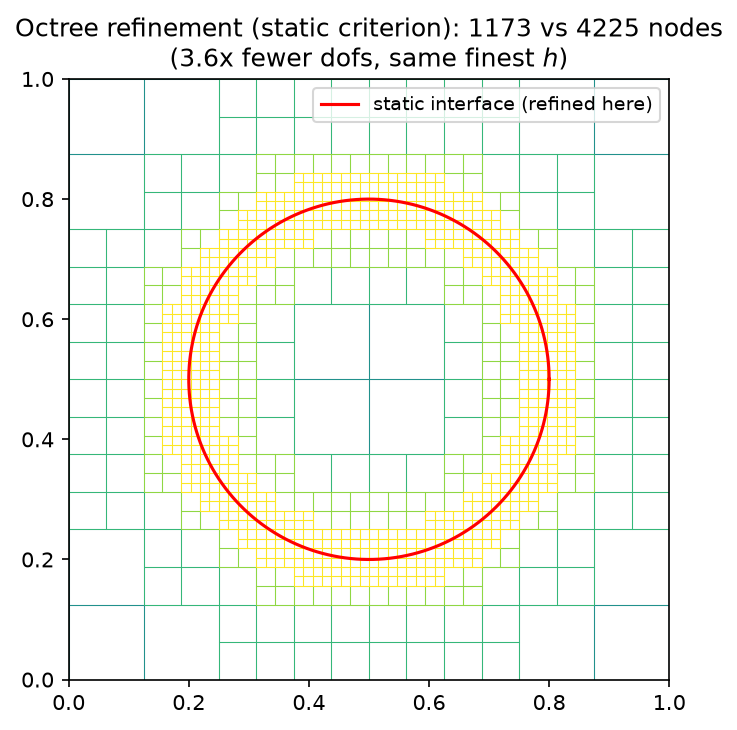
\includegraphics[width=0.6\linewidth]{figures/c3_octree.png}
  \caption{Octree refinement along a \emph{static} circular interface:
    small elements hug the circle, large elements fill the bulk. The mesh
    has $\CthreeAdaptNodes$ nodes versus $\CthreeUniformNodes$ uniform
    ($\CthreeNodeSavings\times$ fewer dofs). Element color is refinement
    level.}
  \label{fig:c3octree}
\end{figure}

\section{What dynamic AMR additionally requires --- and the conservative
transfer that makes it work}

Static refinement is the easy half. \emph{Dynamic} AMR must, every few
steps: \textbf{(a)} estimate the running solution's error, \textbf{(b)}
\emph{mark} elements to refine or coarsen, \textbf{(c)} refine/coarsen,
\textbf{(d)} enforce 2:1 balance (no element more than one level from its
neighbor), \textbf{(e)} rebuild the mesh and the constraint operator
$T$, \textbf{(f)} \emph{transfer} the solution --- \emph{and the BDF
history} --- to the new mesh, and \textbf{(g)} continue the march. Step
(f) is where conservation is won or lost.

\paragraph{Why naive transfer leaks mass.}
When a region is coarsened, the state must be moved to the new mesh
without losing what it represents. A \emph{naive} transfer (inject the
value at the surviving nodes) throws away sub-cell structure and changes
$\intv c$. On a field of droplets smaller than the coarse cell
(Fig.~\ref{fig:c3transfer}), injection loses $\CthreeInjErr$ of the mass
while cell averaging conserves it to $\CthreeAvgErr$. A dynamic-AMR
implementation cannot use nodal injection for the restriction: mass would
leak every time a region coarsens.

\begin{figure}[h]\centering
  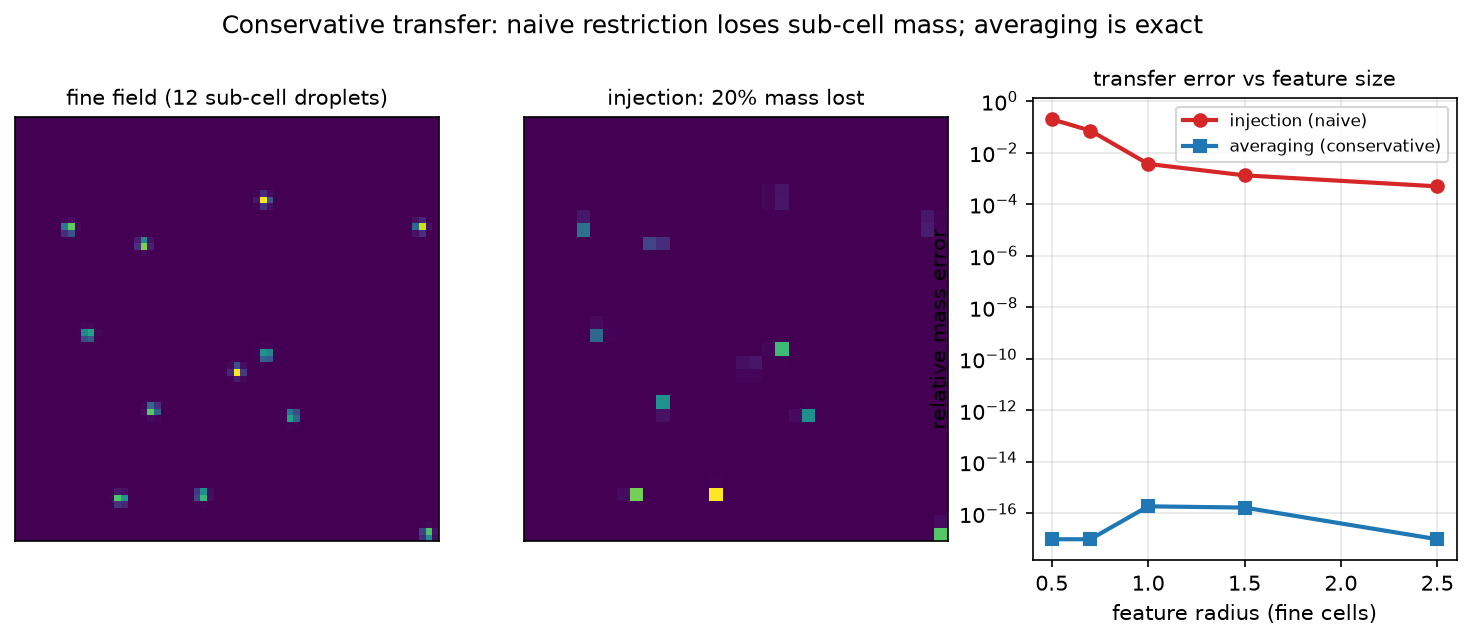
\includegraphics[width=\linewidth]{figures/c3_transfer.png}
  \caption{Conservative transfer, illustrated on a structured grid. Left:
    a fine field of sub-cell droplets. Middle: naive injection to the
    coarse grid misses droplets and loses $\CthreeInjErr$ of the mass.
    Right: injection error grows sharply once the feature drops below the
    coarse cell, while cell averaging is exact at every size.}
  \label{fig:c3transfer}
\end{figure}

\paragraph{The finite-element conservative transfer.}
On an unstructured octree the ``cell average'' generalizes to the $L^2$
(Galerkin) projection with a consistent mass matrix. The subtlety is the
quadrature: to integrate $\int N_a^{\text{new}}\,c_{\text{old}}\,dV$
\emph{exactly}, we integrate on the \emph{common refinement} of the two
meshes --- the finer cell wins in every region --- so both the new basis
function and the old field are linear on each quadrature cell. Because the
finite-element space contains the constant and its basis is a
partition of unity, this preserves $\intv c$ \emph{exactly}: with
$A=T^{\!\top}_{\text{new}} M_{\text{new}} T_{\text{new}}$ and
$b=T^{\!\top}_{\text{new}}\!\int N^{\text{new}} c_{\text{old}}\,dV$,
%
\begin{equation}
  \intv{c_{\text{new}}}
    = \mathbf{1}^{\!\top}_{\text{free}} A\,c_{\text{new}}
    = \mathbf{1}^{\!\top}_{\text{free}}\, b
    = \intv{c_{\text{old}}}.
\end{equation}
%
Measured on the CH brick's meshes: the transfer conserves $\intv c$ to
$\CthreeFeMassRefine$ under refinement and $\CthreeFeMassCoarsen$ under
coarsening (machine precision, \emph{both} directions), it converges at
order $\CthreeFeTransOrder$ against an analytic field, and a
refine-then-coarsen round-trip on a representable field is lossless. The
same operator carries the two BDF history levels $c^{n},c^{n-1}$, each
conserved independently. This is the primitive the cycle below is built on.

\section{Dynamic AMR: the full solution-adaptive cycle}

We now run the whole cycle on a moving interface. The indicator is the
per-element $|\nabla c|$ (large on the diffuse interface, $\approx0$ in the
flat bulk); elements above a fraction of its maximum are marked to refine,
elements below a smaller fraction are marked to coarsen (only complete
sibling groups collapse). After marking we refine, coarsen, re-impose 2:1
balance, rebuild the mesh, constraints and device operators, conservatively
transfer $c$, $\mu$ and both history levels, and continue. The initial
condition is adapted \emph{before} the march --- otherwise the first few
steps run on an under-resolved interface and inject error a uniform-fine
run never pays.

\begin{figure}[h]\centering
  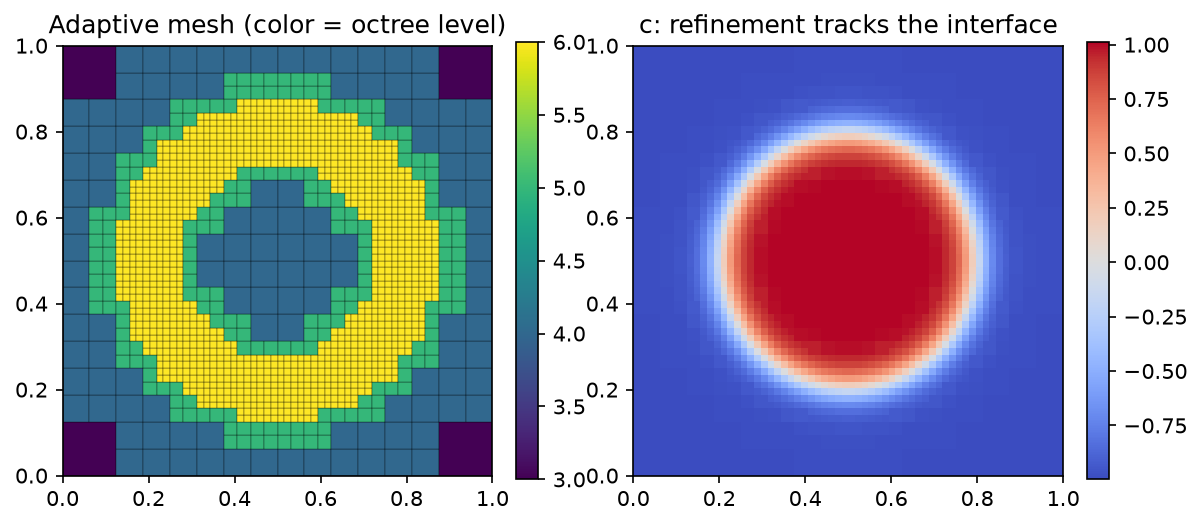
\includegraphics[width=\linewidth]{figures/c3_amr_cycle.png}
  \caption{Dynamic AMR over a shrinking droplet. Left: the adaptive mesh,
    colored by octree level --- the finest cells (level 6) hug the
    interface in a 2:1-balanced annulus grading down to a coarse bulk.
    Right: the field $c$; refinement tracks exactly where the field varies.}
  \label{fig:c3amrcycle}
\end{figure}

\begin{keybox}
\textbf{Measured cycle.} Over the run the march remeshes
$\CthreeAmrRemeshes$ times. Across \emph{every} remesh, $\intv c$ changes
by at most $\CthreeAmrMassJump$ (machine precision), and the free energy
$F$ by at most $\CthreeAmrEnergyJump$ --- the transfer projection error
only, never a spurious jump (Fig.~\ref{fig:c3amrcons}). The refined region
tracks the interface: the overlap between the finest cells and the
interface band is $\CthreeAmrOverlap$. The march stays stable (bounded,
finite) at a peak of $\CthreeAmrDofsPeak$ dofs.
\end{keybox}

\begin{figure}[h]\centering
  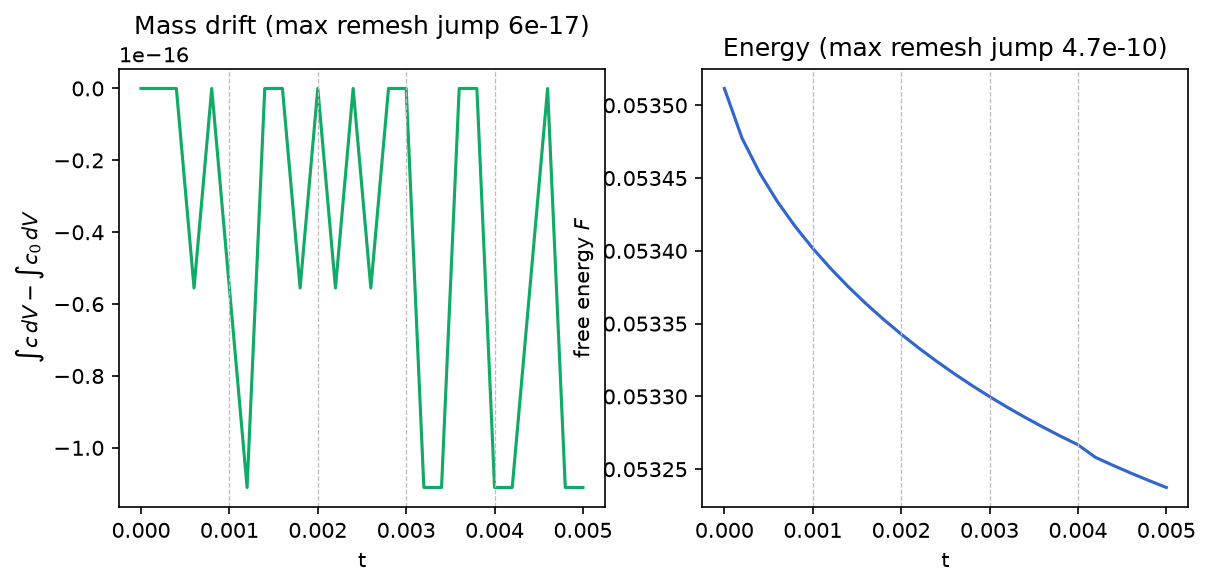
\includegraphics[width=0.86\linewidth]{figures/c3_amr_conservation.png}
  \caption{Conservation across remeshes (dashed lines mark remesh times).
    Left: the mass drift stays at round-off. Right: the free energy is
    continuous across each remesh --- the conservative transfer moves the
    state without a spurious energy jump.}
  \label{fig:c3amrcons}
\end{figure}

\section{Does dynamic AMR pay? Error versus dofs}

Adaptivity is only worth its machinery if it reaches a given accuracy at
fewer degrees of freedom. We score the AMR final state against a
uniform-level-$\CthreeAmrRefLevel$ reference ($\CthreeAmrRefDofs$ dofs) and
compare with a uniform-mesh sweep (Fig.~\ref{fig:c3amrdofs}). Dynamic AMR
reaches error $\CthreeAmrErr$ at $\CthreeAmrDofs$ dofs --- comparable to
the uniform level-$\CthreeAmrFineLevel$ mesh ($\CthreeAmrFineErr$ at
$\CthreeAmrFineDofs$ dofs) but at $\CthreeAmrDofRatio\times$ fewer dofs than
a uniform mesh would need for the same error, and $\CthreeAmrWallRatio\times$
less wall time. The advantage grows with the finest level, because the
uniform mesh pays for resolution everywhere while AMR pays only along the
interface.

\begin{figure}[h]\centering
  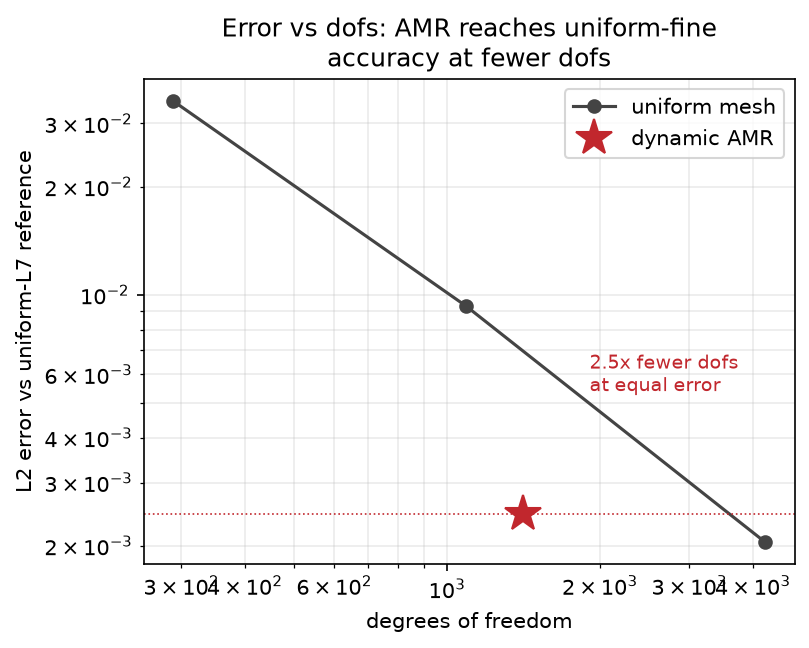
\includegraphics[width=0.6\linewidth]{figures/c3_amr_error_dofs.png}
  \caption{Error versus dofs. The uniform sweep (black) traces the
    accuracy--cost curve; dynamic AMR (red star) sits to its left ---
    uniform-fine accuracy at $\CthreeAmrDofRatio\times$ fewer dofs.}
  \label{fig:c3amrdofs}
\end{figure}

\section{Space-time interaction: a remesh during a BDF2 march}

Dynamic AMR and BDF2 are not independent. BDF2 is a two-step method: its
current step reads $c^{n}$ \emph{and} $c^{n-1}$. When a remesh lands
between two steps, \emph{both} history levels must be transferred to the
new mesh, or the scheme is fed an inconsistent history. We measure the
temporal order of a variable-step BDF2 march that remeshes at its midpoint,
two ways: \textbf{both} (conservatively transfer $c^{n}$ and $c^{n-1}$,
keeping the step-ratio $r=\Delta t/\Delta t_{\text{prev}}$ so the
variable-coefficient BDF2 continues uninterrupted) and \textbf{drop}
(transfer only $c^{n}$ and restart as BDF1 for one step --- the
``only $c^{n}$ is not enough'' failure).

\begin{keybox}
\textbf{Measured order recovery.} Transferring both history levels
recovers order $\CthreeStBothOrder$ across the remesh --- second order
survives. Dropping the second level forces a BDF1 restart; a \emph{single}
restart still recovers order $\CthreeStDropOrder$ (one first-order local
error is $O(\Delta t^2)$, the same size as the global BDF2 error), but it
inflates the error constant by $\CthreeStDropPenalty\times$. The lesson: a
remesh is order-preserving \emph{only} when the full BDF history transfers;
and because the step-doubling controller sees the inflated post-remesh
error as a larger LTE, dropping history also makes the controller shrink
$\Delta t$ needlessly. This is why C1 and C3 are one story.
\end{keybox}

\section{Temporal adaptivity: the LTE step ladder}

Phase separation is violent at onset and glacial during coarsening. A
fixed $\Delta t$ must be small enough for the onset, wasting effort ever
after. The \emph{adaptive} march sizes each step to the physics using a
\emph{local truncation error} (LTE) estimate: it takes one step of size
$\Delta t$ and two of size $\Delta t/2$ from the same state, and the
scaled difference estimates the step error. If it is below tolerance,
accept and \emph{grow} $\Delta t$; otherwise reject, halve, and retry.

Over a quench the accepted step spans $\CthreeDtMin\to\CthreeDtMax$
(a $\CthreeSpan\times$ range, Fig.~\ref{fig:c3ladder}): tiny during onset,
large during coarsening.

\begin{figure}[h]\centering
  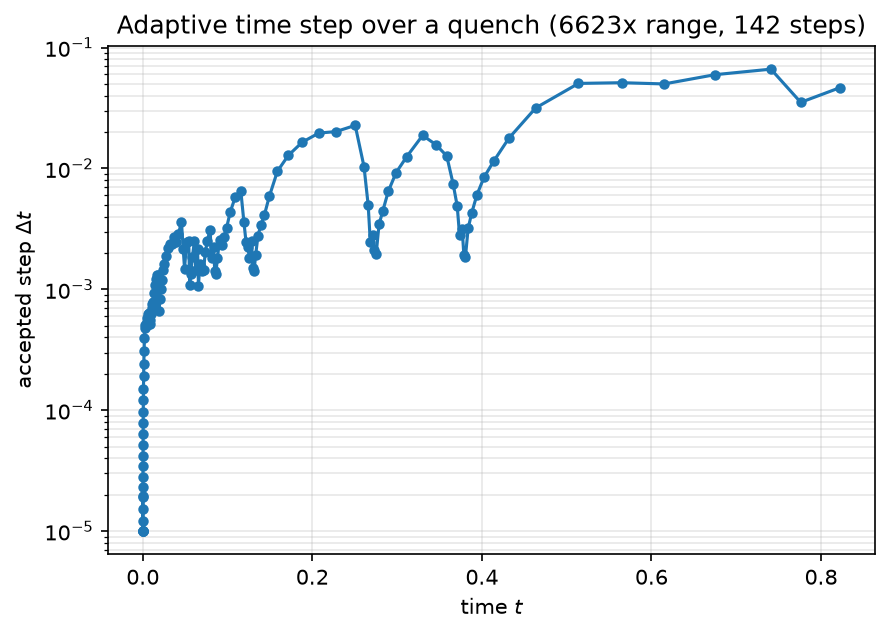
\includegraphics[width=0.72\linewidth]{figures/c3_ladder.png}
  \caption{The accepted time step over a quench (log scale). $\Delta t$ is
    tiny during the spinodal onset and grows orders of magnitude through
    coarsening --- the property that makes long horizons affordable.}
  \label{fig:c3ladder}
\end{figure}

\paragraph{Real cost accounting (not a fiction).}
The honest way to value adaptivity is to \emph{count the work}, not to
multiply the horizon by the smallest step. To reach $t=\CthreeCostTend$ the
adaptive controller took $\CthreeAdaptAccepted$ accepted and
$\CthreeAdaptRejected$ rejected steps --- $\CthreeAdaptSolves$ Newton
solves in all (each accepted step costs \emph{three}: one full plus two
half), $\CthreeAdaptNewton$ Newton iterations, at final error
$\CthreeAdaptErr$. A matched-accuracy fixed-dt sweep finds
$\Delta t=\CthreeMatchedDt$ reaches the same accuracy at
$\CthreeMatchedNewton$ Newton iterations --- so adaptivity saves
$\CthreeNewtonSavings\times$ the Newton work and $\CthreeWallSavings\times$
the wall time here (Fig.~\ref{fig:c3cost}). The saving is real but
\emph{modest}, and it grows with the horizon. This is the honest picture
the old ``horizon / smallest-step'' ratio badly overstated.

\begin{figure}[h]\centering
  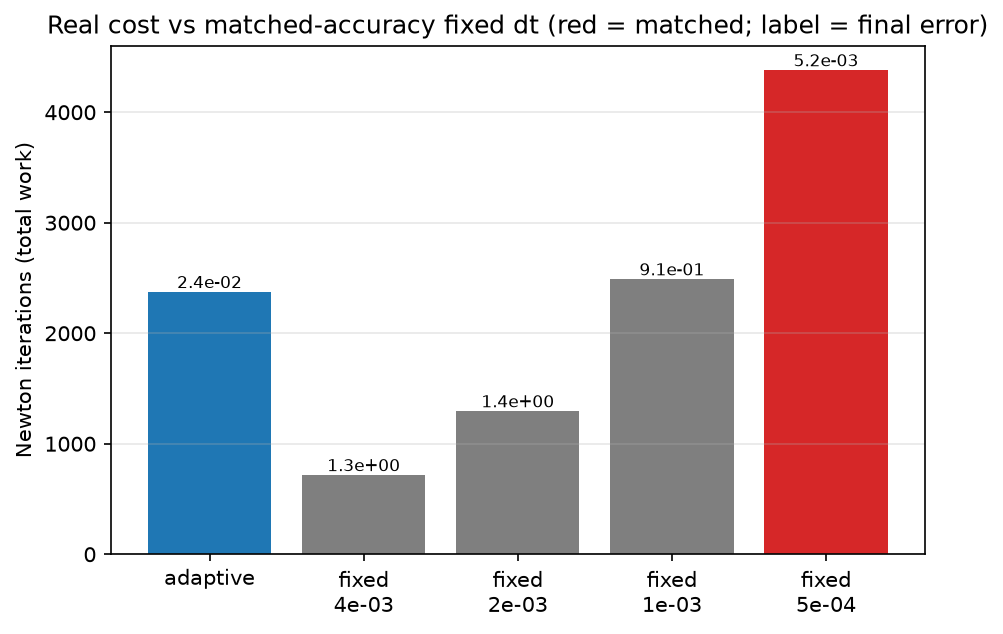
\includegraphics[width=0.72\linewidth]{figures/c3_cost.png}
  \caption{Real cost: total Newton iterations for the adaptive march
    versus the fixed-dt sweep (red = the matched-accuracy fixed run;
    labels are final error). Adaptivity's advantage is measured, not
    assumed.}
  \label{fig:c3cost}
\end{figure}

\section{Why variable-coefficient BDF2}

Growing $\Delta t$ safely has a hidden cost. The textbook BDF2
coefficients $\tfrac32,\,[2,-\tfrac12]$ are derived assuming a
\emph{constant} step. Feed them a step that changed from the last one and
the scheme is only \emph{formally} second order --- its measured order
collapses toward 1. We measure this \emph{here}, with a tutorial-local
constant-coefficient march (we keep the real alternating history spacing
but force the coefficient ratio $r=\Delta t/\Delta t_{\text{prev}}$ to $1$
each step): order $\CthreeConstOrder$. The fix rebuilds the coefficients
each step from the actual ratio,
%
\begin{equation}
  c_0 = \frac{1+2r}{1+r},\qquad
  \text{history weights } \big[\,1+r,\; -\tfrac{r^2}{1+r}\,\big],
\end{equation}
%
which reduces to the constant-step form at $r=1$ and stays consistent when
$r\ne1$. The brick uses it, and the same alternating sequence now measures
order $\CthreeVarOrder$ --- second order restored. It is the \emph{same}
scheme, and the \emph{same} order-preservation requirement, that the
space-time section stressed across a remesh.

\section{Run it}

\begin{runbox}
\textbf{Run it.}
\begin{lstlisting}
cd computational/03_adaptivity
python run.py            # static octree + dynamic AMR + cost + BDF2 order
\end{lstlisting}
Prints the \code{PASS/FAIL} checks. Compare with \file{EXPECTED.md} and
Figs.~\ref{fig:c3octree}--\ref{fig:c3cost}.
\end{runbox}

\begin{keybox}
\textbf{Measured self-check} (fixed seed; node counts are exact, step
counts are seed/card-dependent).
\begin{center}\small
\begin{tabular}{lcc}
\toprule
study & measured & note \\
\midrule
octree nodes (adaptive / uniform) & $\CthreeAdaptNodes$ / $\CthreeUniformNodes$ & $\CthreeNodeSavings\times$ fewer \\
FE transfer mass (refine / coarsen) & $\CthreeFeMassRefine$ / $\CthreeFeMassCoarsen$ & machine precision \\
FE transfer order & $\CthreeFeTransOrder$ & 2nd-order projection \\
AMR remesh mass / energy jump & $\CthreeAmrMassJump$ / $\CthreeAmrEnergyJump$ & conserved / continuous \\
AMR interface overlap & $\CthreeAmrOverlap$ & refinement tracks interface \\
AMR error vs dofs & $\CthreeAmrDofRatio\times$ fewer & at equal error \\
remesh order (both / drop history) & $\CthreeStBothOrder$ / $\CthreeStDropOrder$ & order 2 preserved \\
adaptive Newton saving & $\CthreeNewtonSavings\times$ & modest, grows with horizon \\
BDF2 order (variable / constant) & $\CthreeVarOrder$ / $\CthreeConstOrder$ & order preserved vs collapsed \\
\bottomrule
\end{tabular}
\end{center}
\end{keybox}

\section{Code walk-through}

\paragraph{The dynamic-AMR cycle (the Phase-3 core).}
\begin{lstlisting}
ind = interface_indicator(stepper, mesh)      # |grad c| per element
refine_mask, coarse_mask = mark(tree, ind, ...)
new_tree = adapt_tree(tree, refine_mask, coarse_mask)   # +2:1 balance
stepper, mesh, cons = remesh(stepper, mesh, cons, new_tree, ...)
# remesh conservatively transfers c, mu AND both BDF history levels
\end{lstlisting}

\paragraph{Conservative transfer (the piece AMR needs).}
\begin{lstlisting}
conservative_transfer(mesh_old, cons_old, tb, mesh_new, cons_new, tb,
                      [c, mu, hist0, hist1])   # L2 proj on common refinement
\end{lstlisting}

\paragraph{Real cost accounting.}
\begin{lstlisting}
instrumented_march(st, t_end, tol)   # counts acc/rej, solves, Newton, wall
adaptive_cost()                      # + matched-accuracy fixed-dt sweep
\end{lstlisting}

\paragraph{Constant- vs variable-coefficient BDF2 (both measured).}
\begin{lstlisting}
_var_march(dm, dt)     # brick: coefficients from the real r = dt/dt_prev
_const_march(dm, dt)   # forced r=1 on a varying history -> the bug
\end{lstlisting}

\section{Explore on your own}

\question{Change the refinement indicator from $|\nabla c|$ to a
gradient-jump (the difference in $\nabla c$ across element faces). Does the
refined region still track the interface? Which indicator marks fewer
cells for the same final error?}

\question{Coarsen more aggressively (raise the coarsen fraction) and watch
the free-energy jump across remeshes. At what point does the coarsening
transfer error stop being negligible --- and does 2:1 balance re-refine the
region you tried to coarsen?}

\question{Extend the cost accounting to $t_{\text{end}}=1.2$. Does the
adaptive Newton saving grow (the coarsening tail lengthens)? Plot the
saving versus horizon and find where adaptivity first pays for its
step-doubling overhead.}

\question{In the space-time study, remesh \emph{every few steps} instead of
once. With ``drop'' (a BDF1 restart at every remesh) the number of
restarts now grows as $\Delta t\to0$ --- predict and then measure what
happens to the global order, and contrast with ``both.''}

\question{Force the constant-coefficient bug back on a \emph{fixed}
$\Delta t$ ($r\equiv1$) and confirm you recover order 2 --- then argue why
the alternating sequence, not the fixed one, is the test that exposes the
variable-coefficient issue.}
